\documentclass[12pt, a4paper]{article}
\usepackage[utf8]{inputenc}
%\usepackage[latin1]{inputenc} 
\usepackage[english]{babel} 
\usepackage[T1]{fontenc} 
\usepackage{amsmath,amssymb} 
\usepackage[table]{xcolor}
\usepackage{verbatim}
\usepackage{graphicx}
\usepackage{fancyhdr}
\usepackage{wrapfig}
\usepackage{gauss}
\usepackage{xfrac}
\usepackage[page]{totalcount}
\usepackage{caption}
\usepackage{subcaption}
\usepackage{booktabs}
\usepackage{setspace}
\usepackage{enumitem}
\usepackage{placeins}
\usepackage{hyperref}
\usepackage{titlesec}
\usepackage{multirow}
\usepackage{epigraph}

\usepackage{multicol}

\setlength{\headheight}{15pt}

\titlespacing\section{0pt}{12pt plus 4pt minus 2pt}{0pt plus 2pt minus 2pt}
%\setcounter{tocdepth}{3}
%\setcounter{secnumdepth}{3}
%\setcounter{secnumdepth}{0}

%marginer
\usepackage[top=2.5cm, bottom=2.5cm, left=2.5cm, right=2.5cm]{geometry}


% patch gauss macros for doing their work in `align'
% and other amsmath environments; see
% http://tex.stackexchange.com/questions/146532/
\usepackage{etoolbox}
\makeatletter
\patchcmd\g@matrix
 {\vbox\bgroup}
 {\vbox\bgroup\normalbaselines}% restore the standard baselineskip
 {}{}
\makeatother
\newcommand{\BAR}{%
  \hspace{-\arraycolsep}%
  \strut\vrule % the `\vrule` is as high and deep as a strut
  \hspace{-\arraycolsep}%
}

\pagestyle{fancy}

%subsections get indexed with letters
%\renewcommand{\thesubsection}{\thesection.\alph{subsection}}

%Navn og dato
\lhead{Philosophy of Science}
\chead{University of Copenhagen}
\rhead{\today}

\cfoot{Page \thepage\ of \totalpages}


%begynd dokumentet
\begin{document}
%\begin{spacing}{1.213}



\title{ Philosophy of Science  \\ \Large Course notes \\ \normalsize \today \\ 
%\normalsize {No. of signs: }
} 
\author{\normalsize Kristian Urup Olesen Larsen}
\date{} % Use current date.
\maketitle % Print title page.
\pagenumbering{roman} % Roman page number for toc
\setcounter{page}{1} % Make it start with "ii"

%\chapter{A Main Heading} % Make a "chapter" heading
\pagenumbering{arabic} % Start text with arabic 1

%---------------------------------------------------------------
%-------SKRIV HERUNDER----------------------------------
%---------------------------------------------------------------

\epigraph{"Spoon feeding leads to regurgitation"}{\textit{Thomas Barnebeck Andersen}}
\tableofcontents
\pagebreak

\begin{multicols}{2}
\section{Part 1: Schools of Thought in PoS}

\subsection{Intro}
Science is the systematic endeavour to develop and organize knowledge of the world, in the form of testable/predictable explanations. PoS is concerned with the way in which we do this. 

Scientific realism is a belief that "science works", that is science produce true theories, which are concerned with real things. It is believed that scientific progress converges to a truth. 
\begin{itemize}
\item Science discovers new truths
\item Enough evidence proves that theories are true
\end{itemize}
Antirealists hold that while theories might be useful, they dont actually represents the true nature of things. Most notably is the empiricists, which say that empirical evidence is knowledge/truth in itself, contrary to the realists who claim that evidence support and can prove the state of underlying unobservables.

\paragraph{Phenomena} are empirical regularities, often understood as causal effects, which of course can only be inferred to exist through the trace they leave in the measurements we can make. 

Scientists formulate abstractions that highlight the underlying causal mechanisms - often in a stylized way.
\epigraph{"Economics has three goals; explanation, prediction and control"}{\textit{Carl Menger}}

\subsection{Logical positivists - Popper, Kuhn}
Logical positivism became a prominent position in PoS during the 20th century, often attributed to the so called \textbf{Vienna Circle}. Their main goal was to find useful distinctions between science and pseudo-science. 

\begin{itemize}
\item Logicism: ~ any language is an extention of logic
\item positivism: ~ knowledge arises from sense experience
\item Demarcation rule: ~ accept only analytic and "synthetic a posteriori" statements as scientific knowledge
\begin{itemize}
\item A synthetic statement is one that is not analytic
\item it is synthetic a posteriori if shown true by empirical research ("our dog is aggressive, because we've experienced it" is synthetic a posteriori)
\end{itemize}
\item analytic propositions ~ are true by default (all bachelors are unmarried or 1+1=2)
\end{itemize}
To sum up the logical positivists hold that only verifiable (or intrinsically verified) statements are true science. However how verification should be done is not trivial
\begin{itemize}
\item[1)] how do we verify statements about individuals ("my hair is brown")
\begin{itemize}
\item by direct observation
\end{itemize}
\item[2)] how do we verify generalizations ("all swans are white")
\begin{itemize}
\item By induction 
\end{itemize}
\end{itemize}

\paragraph{The problem of induction} is that it doesn't necessarily hold in all generality. Principles are a good example of why induction sometimes falls short: It's impossible to deduce principles, as they are just conventions, however it's equally hopeless to prove a principle by induction, as they by definition can be changed. 

The main response to the criticism is that usually the probability of a statement being true increases with the number of times it's been observed. 

\subsubsection{Karl Popper}
Popper rejects classical inductivist views in favor of falsification $\rightarrow$ a scientific theory can never be proved, but it can be falsified. According to him we can never actually prove theories, science is not about establishing truths, as theories are always just (qualified) guesses. Instead science is about choosing between theories, which is why falsification is a good tool. Science is demarcated by the requirement that theories are falsifiable (a black swan falsifies the claim that all swans are white). 
\begin{itemize}
\item some politicians are often wrong is not falsifiable
\item All women wear lipstick is falsifiable
\end{itemize}
Popper suggests a \textbf{immunizing stratagem} as a sign that theories are unscientific. If theories can incorporate whatever observation into its framework, it's immune to falsification. (a good example is Freuds theory on denial - "if you say you're not in denial, you only do so because you're in denial"). Thus scientific theories must potentially be incompatible with observables.

Popper acknowledge that with the development of technology unscientific theories might become testable, and thus scientific. To him knowledge arises from the \textbf{leaps of immagination} required to formulate new theories, as old ones are falsified. One can think of this as deductive testing of theories. 

\subsubsection{The Duhem-Quine thesis}
Falsification is not a clean cut between science and non-science. Why? - to test and potentially falsify a claim we need to make background assumptions. If a theory is "proven" false, this can always be blamed on instruments etc. Poppers answer is that because this allows essentially anything to be blamed for a "mis-falsification" it is in itself a immunizing stratagem. 

\subsubsection{Thomas Kuhn}
Introduced the notion of \textbf{paradigm shifts}. Instead of attempting to define what science is and should be, he developed a positive/descriptive explanation. 
\begin{itemize}
\item Kuhn's central argument is that in normal periods, as scientific field follows a paradigm/thought pattern. 
\begin{itemize}
\item When a paradigm proved unable to produce explanations to anomalies a scientific revolution occurs. 
\end{itemize}
\item His \textbf{incommensurability thesis} states that it's meaningless to compare theories developed under different paradigms.
\end{itemize}
In "normal" science, research builds on previous results and ideas, and is based around a number of seminal articles ("classics" in the field). With a paradigm follows textbooks and researches pursuing the same questions with the same methods. Thus "normal" science is a puzzle solving exercise. Scientists who doesn't adhere to the paradigm are marginalized. 

While there might be problems that cannot be solved under a paradigm, these problems are simply ignored. When however these anomalies show up, the paradigm is modified to accommodate, but as the paradigm proves insufficient the paradigm must change. It's important to distinct between the falsifications of Popper and Kuhn's anomalies however, as Kuhn suggests that paradigms can continue for some time in an attempt to understand the anomalies. Additionally falsification is concerned with single statements, not entire fields of science. \textbf{It lies implicitly in Kuhns work that the object of study stays the same, while the perspective from which it is seen changes.}

\subsection{Lakatos and the rethoric of economics}
\subsubsection{Imre Lakatos}
Lakatos is known for his theories of \textbf{sophisticated falsificationism (SF)} and his concept of \textbf{research progammes (RP)}. He critiques Kuhns idea of paradigm shifts, as Kuhn doesn't offer a rational explanation as to when a paradigms shift should occur. To Lakatos Kuhn's notion of scientific changes is similar to that of religious changes, that is irrational and governed by a mystical convention. Instead Lakatos tried to defend Poppers ideas about scientific growth by unifying the theory of Kuhn with that of Popper, through SF and RP.

\paragraph*{Research programmes}
\begin{itemize}
\item have two elements:
\begin{itemize}
\item a core of theoretical assumptions that cannot be altered or abandoned without abandoning the programme altogether
\item More modest theories that seek to explain evidence that threatens the core - auxiliary hypotheses. These auxiliary hypotheses can be altered or abandoned to accommodate evidence that would otherwise threaten the core. 
\begin{itemize}
\item Popper: would not like these, they resemble immunizing stratagems
\item Lakatos: they can advance the predictive power of a theory, and we can live with them until a stronger research programme is invented/discovered
\end{itemize}
\item are a sequence of theories within a scientific field
\end{itemize}
\item Problem shifts happen through SF. New RP's should be measured against the predecessor.
\begin{itemize}
\item Attempts at falsification should be directed towards the non-core theories.
\end{itemize}
\end{itemize}
\paragraph{Sophisticated falsificationism}
\begin{itemize}
\item Instead of abandoning theories as soon as they're falsified (as Popper would like it), Lakatos suggest that a theory $T_1$ should be abandoned in favor of another theory $T_2$, if 
\begin{itemize}
\item $T_2$ has excess empirical content compared to $T_1$, that is $T_2$ makes novel predictions.
\item $T_1^+ \in T_2$, that is all unrefused content of $T_1$ is in $T_2$
\item some of the excess content of $T_2$ is confirmed by experiment or observation.
\end{itemize}
\end{itemize}
So the major differences between Popper and Lakatos is that while Popper claims that scientists attempt to falsify theories, Lakatos says that they 1) modify existing theories by proposing better alternatives, 2) test the predictions of novel alternative theories and 3) reject existing theories when some predictions of the new theory are substantiated through evidence. Lakatos shifts the focus from single theories to sequences of theories (RP's and their evolution).

A final major difference is that while Popper says that theories that have proven successful under harsh testing should be scrutinized even more closely; Lakatos says that theories that survive harsh testing should be considered as "more true" (verisimilitude is increasing in testing).

Finally Lakatos makes a distinction between RP's that are progressive, and those that are degenerative, based on whether recent changes to a RP has increased the predictive power of the theory or function as immunizing strategies. When a RP becomes degenerative the search for a successor should begin. Until an agreement on a new RP can be made, it's however better to keep the old RP, to not loose predictive abilities while the new RP develops. Even when we know a theory cannot be completely true, it is better to continue developing it, as long as we stay receptive to better alternatives.

What Kuhn described as paradigm shifts, Lakatos would thus instead decribe as periods in which a better RP supersedes a more progressive RP. 
\subsection{Friedman and the methodology of positive economics}
\subsubsection{Milton Friedman} 
Friedman is concerned with issues that arise in the attempt to make economics a "distinct positive science", specifically when to consider a hypothesis as part of the "body of systematized knowledge concerning what is". He realizes that many policy disputes aren't disputes over basic values, but rather disputes over the consequences of certain or alternative actions. Therefore positive economics can provide answers and solve disputes.

\epigraph{"The ultimate goal of a positive science is the development of a theory or hypothesis that yields valid and meaningful predictions about phenomena not yet observed"}{\textit{Milton Friedman}}
The issue then is that economics have few natural experiments, and thus it's hard to draw hard conclusions even with a large body of empirical evidence. The alternative has been to formulate "realistic" assumptions instead, something Friedman thinks is a grave mistake. Instead theories should be measured by their ability to predict, no matter how unrealistic their assumptions are. When choosing which hypothesis to use, one should be guided by 
\begin{itemize}
\item The simplicity of the hypothesis
\begin{itemize}
\item a simple hypothesis requires less initial knowledge to make predictions
\end{itemize}
\item The fruitfulness of the hypothesis, in terms of predictive power
\begin{itemize}
\item a fruitful hypothesis is one that is better at predicting, can make a broader range of predictions and/or provides more paths for further research.
\end{itemize}
\end{itemize}
For a hypothesis to be logically complete and consistent is important but secondary. The main purpose of logic and consistency is to ensure that hypotheses are formulated correctly and precisely.
\epigraph{"Economists have supposed that they could test theories by the realism of their assumptions rather than by the accuracy of their predictions"}{\textit{Milton Friedman}}
Thus a good measure of the importance of a hypothesis according to Friedman is that is explains "much by little". One should not expect of assumptions to be realistic, but rather for them to be good at predicting $\Rightarrow$ the only way to validate assumptions is to use them for prediction. 


This also mean that theories should only be judged for their purpose, that is in the narrow domain they're intended to explain.

\paragraph{criticism} of Friedmans ideas is broad. On a very simple level, one might disagree that the only purpose of economics is prediction. As scientists we also want to understand and explain the mechanisms driving our results. General Equilibrium models are often suggested as examples of Friedmans ideas, as they build only on the necessary conditions for establishing a pareto-optimal, unique and stable equilibrium of prices and quantities. 
\epigraph{"unlike any scientific theory, where the basic assumptions are chosen on the basis of direct observation of the phenomena the behaviour of which forms the subject-matter of the theory, the basic assumptions of economic theory are either of a kind that are unverifiable-such as that producers “maximise” their profits or consumers “maximise” their utility - or of a kind which are directly contradicted by observation – e.g, perfect competition"}{\textit{Kaldor}}
\subsubsection{P. Samuelson - The descriptivism debate}
Samuelson interprets Friedmans ideas as the position that a theory is supported(/able) if it's predictions are empirically valid to a useful degree of approximation. And further that the empirical unrealism in itself, or in it's assumptions is irrelevant, when judging the worth of a theory.

Samuelson himself however considers strict unrealism (as in factual incorrectness) a scientific sin. He calls Friedmans view the F-twist as it, according to him, allows theories importance although the theory itself might be completely wrong, albeit good at prediction. Instead he assumes a descriptive position, where a valid system is equal to its \textit{complete} set of empirical consequences - which all should be tested. This implies that theories cannot provide explanations but only descriptions.
This position has received critique as the complete set of consequences is simply to large to be tested. 

\subsection{explaining economic phenomena}
Explaining phenomena is a core aim of economics. We do this by proposing hypotheses/models/"stories" to explain phenomena of interest. Recall
\begin{itemize}
\item A phenomena is detected through the use of observable data, but is not in itself observable. Instead it is inferred to exist on the basis of data. Phenomena are thus
\begin{itemize}
\item (usually unobservable but) measurable
\item of scientific interest
\item to be inferred from data
\item to some extend idealized
\end{itemize}
\end{itemize}
In explaining phenomena we ask "why?" questions which we answer with valid scientific methods. We call the thing to be explained the \textbf{explanandum}. The sentences/arguments used to explain the explanandum are called the \textbf{explanands}. Thus to a logical positivists, the "correct connection between explanandum and explanands is that of "logical consequence" i.e. if A, if B then always C would be considered a valid explanation of C.

\subsection{The D-N model and its discontents}
The D-N (deductive nomological) model of explanation is a formulation of how good explanations should look like. It consists of true statements of initial conditions (C), scientific laws (L) and deduces from those an explanandum. As an example consider 
\begin{itemize}
\item[$C_1$] X is a monopoly firm
\item[$C_2$] Marginal costs has increased
\item[$L_1$] All monopolies increase prices if marginal costs increase
\item[$\Rightarrow$] Firm X increased its prices
\end{itemize}

\paragraph{A scientific law} is, according to the logical positivists not clearly defined. But can be loosely defined as "universal generalizations", which are contingent(not true in themselves), verifiable and supported by evidence. Attemps at formally distinguishing scientific("nomological") laws from accidental ones (like "all pages in my notebook are blank") have so far failed.

Another option would be to define laws by listing paradigms, such as \textit{the law of diminishing returns} and \textit{the laws of supply and demand}.

\paragraph{Critique of the DN model} can be as simple as $C_1:$ George takes birth control pills, $L_1:$ People on birth control doesn't get pregnant $\Rightarrow$ George doesn't get pregnant.

More sophisticated critique exists, first of the idea that generalizations are strictly universal is often not true, and thus laws often doesn't express universal generalizations but \textit{ceteris-paribus} statements or (causal) tendencies. Secondly what appears to be laws might actually be explanands themself - the law "all monopolies increase prices when marginal costs increase" is not so much a law as a question that need answering. Thus good economic explanations should shed light on the causal mechanisms 

A substantial final critique is that DN implies symmetry, that is if something can be shown to be caused by some variables, it is reversible so that the previously explaining variables can be considered causes themself, in other words if we can show $C+L \Rightarrow E$ it is reversible to $C \Leftarrow L + E$
\subsection{Causality} \label{seq: causality}
Naturally we cannot observe the causal relationships linking causes to their effect, and thus by Humes "what we cannot see, we cannot know" we would not be able to know causal relationships. This skepticism is shared by the logical positivists. if one holds these beliefs, it will however cost the ability to provide explanations and policy solutions. 
Unlike the ideas formulated in the DN model, causation is asymmetric, that is cause only goes one way. Hume (somewhat outdated) formulates causation of the form "X causes Y" as being true when
\begin{itemize}
\item X is universally associated with Y
\item Y follows X in time
\item X and Y are spatio-temporally contiguous (no gaps in time/space between X and Y)
\end{itemize}
\paragraph{John S. Mills} considers economic laws as tendencies at best, by which he means that economic laws does not so much explain outcomes, as they explain a trend whereto outcomes generally abide in the absent of disturbing forces. One way of formulating this is that causal tendencies are:
\begin{itemize}
\item[] kinds of causes, which produce a stable and characteristic effect when operating in the absence of disturbing forces, but continue to contribute to outcomes when disturbing factors are present.  
\end{itemize}
This definition is not totally fulfilling either, in part because establishing such regularities does not necessarily carry explanatory power. Instead we should seek out to understand why this regularity hold, that is we should describe \textbf{causal mechanisms} that ensures that a regularity continues to hold. One can think of mechanisms as connecting causes and effects. The thinking of mechanisms and how they work is highlighted in economics through the debate of methodological individualism, the idea that we should model the world as being constructed on basis of the interactions of individuals.   
\section{Part 2: Economic Rules}

\subsection{What models do}
Economics is an important science for real life events, and misuse of economic science can have great implications. 

Unlike in physics there is no ultimate model in economics - instead we expand our \textbf{library of models} to better suit the situations we encounter. The craft of selecting correctly among models is crucial.

To Rodrik the critique of economics is often misguided, as it fails to realize that economy as a science is a library of models, not the search for a ultimate (ideologically biased) model.

\textbf{At least two definitions of 'economics'} are commonplace, namely 
\begin{itemize}
\item The social science devoted to understanding how the economy work.
\item A way of doing social science using tools such as mathematics and statistics. (Rodriks definition)
\end{itemize}

\textbf{What do models do?} - they are used for their simplicity and formalism. They purposely neglect real world details. They exist in many shapes and sizes, and when used correctly they illuminate our understanding. When used dogmatically it leads to hubris and bad policy advice.

Usually models are used to study a widely defined variation of market outcomes, and allocations in such situations. 

Imagine for example a situation where a bus drives around Uganda supplying HIV-tests to sex workers. We know that the price of safe sex is less than that of unsafe sex, but we need a model to understand what happens to the supply of unsafe sex, when we introduce the bus. 

\subsubsection{Models as fables}
We can think of models as "stories" or fables (stories with few characters, whose interactions serve as lessons to the reader). Both sacrifice realism for clarity, and both offer a transparent moral.
\epigraph{"The word 'model' sounds more scientific than 'fable' or 'fairytale' yet there is not much difference between them"}{\textit{Ariel Rubenstein}}
The idea that models in some way are stories have been reiterated by many including: "An economic model always tell a story" (Hal Varian).

There exist many fables, so we use our judgement in selecting the right ones for a given situation. This is exactly as with economic models. 

\subsubsection{Models as experiments}
Models can also be thought of as experiments, where each model is equivalent to a "lab setup". Thus models allow us to carefully study the causal effects in a model world. This of course implies a lot of internal validity for model "experiments", but probably not a very high external validity. 
This raises the question of whether assumptions need to be realistic -> reacall Friedmans opinion (and critique thereof).

Rodrik argues that a realism filter must be applied to the assumptions economists make. He makes the distinction of \textbf{critical assumptions}, which are defined as being assumptions that if changed in a more realistic assumption, produces significantly different outcomes. Thus what makes an assumption critical depends also on what the model is used for. Rodrik says that unrealistic assumptions are ok, but not of they're critical.

\subsubsection{Math and models}
Math raises a \textbf{comprehensibility barrier} between economics and other social sciences. According to Gerring these kinds of barriers are detrimental to the argument that we should have publicly funded researchers, because for the public to gain from research it must be understandable.

On the other hand, math provides clarity about arguments and consistency in conclusions. All in all this points to a tradeoff between simplicity and complexity on a number of levels. 



\subsection{The science of economic modeling}
Models are roughly speaking what makes economics a science, but unlike the physical sciences we're not looking for a single all-explaining model, but rather building a library of models where each model relates to the real world. Economics is a social science, so there are no fundamental laws that will always hold true. That is we have agency (choosers) i.e. humans who choose how to interact in society. 

Models clarify hypotheses and ensures that we avoid slips in intuition. They allow slow and steady accumulation of knowledge that can horizontally evolve the science, and they allow us to make clear testable distinctions between seemingly identical theories. Finally models ensure a universal standard for sharing knowledge within the profession of economics. 

Most models (think of the 1.st welfare theorem) are highly abstract, and lay out foundations for understanding real worlds phenomena, thus to apply them to the world around is we need to perform a \textbf{leap of faith}. However when used correctly they can not only show us how to test our hypotheses, but also warn of potentially unwanted consequences. An important note to make here, is that of the \textbf{second-best option theorem} which shows that if one optimum condition cannot be satisfied, other optimum conditions will generally change as well. I.e. if we cannot achieve the ideal interest rate, this will also force our previous solution for the tax-rate to change. 

\epigraph{"The world is second-best at best"}{\textit{Avinash Dixit}}

The second-best theorem has widespread consequences; think of the Washington consensus (10 'rules' to follow for developing countries/countries in crisis according to the IMF, WB etc. - basically a prescription of liberalization), this might not be so true, if one of the goals is unachievable for the specific country. 

In economics we rarely make vertical advances (that is we rarely replace old theory with new ones), instead we advance horizontally. Whenever a theory cannot explain a certain phenomena we simply construct one that can. We introduce an element of \textit{induction}. Instead of postulating how empirics should be if our theories are right, we simply fit our postulated models to the data as good as we can, often soon to be followed by similar studies with opposing results. This calls into question the usefulness of our empirical approach, compared to the idea of comparing situations to history. Some might say there's an element of fashion in the preferred modeling framework at a given time. To counter the critique, one could say that the essence of society makes it impossible to devise ever-lasting models, and likewise impossible to test models once and for all - to use economic models properly we should understand that context is key. A good example of the horizontal evolution of economics is the study of markets: Perfect competition $\rightarrow$ Imperfect competition $\rightarrow$ asymmetric info $\rightarrow$ behavioral economics. This path has supplied us with a library of models, that fit a broad range of situations where markets are involved.   

Perhaps the most important example of how models allow us to structure and test arguments is the debate of \textit{austerity} vs. \textit{keynesianism}. The Austerions postulate that cutting budget deficits is the only way to prevent bond holders from increasing interest rates, and thereby causing more harm. Keynesianists on the other hand would state that the fiscal multiplier increases in depressions, why government spending is good in these situations. (with models we can test these claims).

In terms of what becomes accepted as scientific contributions comes down to a (sometimes shady) peer-review process that will uncover the quality of a paper, and ones ability to follow the "\textit{rules of engagement}" within the scientific discussion - this goes both when submitting and critiquing).

\subsection{Navigating among models}
For economics to be a useful science we need to apply models properly - thus we need to learn the skill of selecting the right model. As it is now universities doesn't train students in selecting among models, but only provides students with an array of models to choose from. When we ask 'what is the underlying model' we essentially want to know '\textit{what is the dominant causal mechanisms behind the phenomena we observe}'. In a sense this often becomes a matter of identifying \textbf{binding constraints}.
\\ \\
If we lived in a world with no binding constraints, economics would be a matter of tuning each parameter of interest independently of other parameters. In a world with constraints, we need to know which knobs to turn at which times, in order to get the desired outcome. 
\\ \\
A simple way to imagine the extremes of these two cases is to consider a barrel full of water. The barrel is made up of wooden boards, that can either be vertical or horizontal, representing a constrained or not-constrained world. If we're in the unconstrained world (horizontal boards) we can increase the volume of our barrel by increasing the height of any of the boards. If however we're in the fully constrained world (vertical boards) the lowest board is the only one we can heighten to increase volume. This of course only goes until the before-lowest board becomes so high that another one takes its place. 

\epigraph{"One of my favorite Keynes quotes comes from Essays in Persuasion, in which he tried to explain the nature of the Great Depression, which was still in its early stages, and declared that \textit{'we have magneto trouble'}. The economic engine was as powerful as ever — but one crucial part was malfunctioning, and needed to be fixed. That’s about where we are now."}{\textit{Paul Krugman}}

Growth diagnostics is the act of diagnosing why growth has slowed or what will cause it to do so. Depending on ones favored model or ones interests, people will choose different ways of viewing the world, some options are
\begin{itemize}
\item Solow/neoclassical growth models: $L,K$ and $H$
\item Dual economy models: structural transformation
\item Institutions fundamentalism: property rights
\end{itemize}
A real time example of growth diagnostics can be observed after the financial crisis. Although most informed observers expected a quick recovery, we ended up with almost 6 years of near-zero interest rates in the US, negative rates in Europe and QE. What happened has been called \textit{secular stagnation} (SS) - the combined increase in propensity to save, with decreasing propensity to invest. This induced lower demand and interest rates. While this is consistent with the hypothesis that excessive pre-crisis savings was at the root of the crisis, it should also have resulted in a inflation pressure in 03-07 (maybe better inventory management, the rise of China and globalization could have kept this down).

The conceptual framework of SS is that the real interest rate $r$ adjusts to balance savings $S$ and investments $I$. Specifically a natural interest rate $r^n$ balances $S$ and $I$ at full employment. SS is then the notion that $r^n$ became so low that CB's cannot achieve it, for example if $i \in \mathbb{R}_+$ and $\pi^e = 0.02$, then by $r=i-\pi^e$ when $r^n < -0.02$ we have SS and $S>I$.

Of course there are other valid explanations to explain a high $S$ and/or low $I$ on their own. For example inequality would shift income to the rich who save more, or the new sharing-economy conserves capital and thereby reduced the need for $I$ - however SS has the nice feature of falsification, specifically "\textit{A sudden pickup in inflation would do the job}" (Larry Summers).

\subsubsection{Principals of model selection}
Selecting a model is the skill of moving back and forth between candidate models and the real world - a.k.a \textbf{verification}. There are 4 primary ways of verification, namely 
\begin{itemize}
\item[1)] Verifying critical assumptions
\begin{itemize}
\item Crit. assumption $\approx$ assumptions that when changed alters the results drastically
\item Often a crit. assumption: "firm A has market power" $\rightarrow$ we verify this by studying 
\begin{itemize}
\item[a)] Number, size, distribution of firms in the business 
\item[b)] ease of entry
\item[c)] substitution options
\end{itemize}
\end{itemize}
\item[2)] Verifying that the postulated mechanism(s) is(/are) actually operating
\begin{itemize}
\item A mechanism(/causal relation) could be "lower supply increases prices causally" - we test this by
\begin{itemize}
\item[a)] Trying to find places where $if \ A \ then \ C$ is not required, either $if \ A \ not \ C$ or $not \ A \ then \ C$.
\end{itemize}
\end{itemize}
\item[3)] Verifying the direct implications of the model (similar to (2))
\item[4)] Verifying incidental (derived/implied) consequences of the model
\begin{itemize}
\item Models provide more implications than the key ones - we can test those instead of the key implications
\end{itemize}
\end{itemize}


\subsection{Models versus theories}
Models are not the same as theories, whereas models are designed to provide partial and idealized answers in the study of causal mechanisms, theories are on the other hand ambitious, general and of near-universal validity (think of the 'theory of general relativity'). Put simply models answers \textit{what?}-questions, whereas theories answer \textit{why?}-questions. Often theories in economics do not seek to generalize i.e. the 'theory of the financial crisis', but rather to explain specific phenomena. Models scrutinize $X \rightarrow Y$ causal relations. Thus there is an important distinction between what could be called \textbf{forward- and reverse causal inference}. 

\begin{itemize}
\item Forward inference, is what we use when building models from $X \rightarrow Y$ relations
\item reverse causal inference is what we use when constructing theories: after examining all possible explanations we select between them to produce a probable large-scale phenomena for what we observe i.e. 'selecting models from the library'.
\end{itemize}

\paragraph{Grand theories} are timeless questions like 'what determines the distribution of income' or 'is capitalism stable', but ever so often these kinds of questions are impossible in the social sciences because of the ever changing nature of societies. These are called \textbf{universal and non-contextual} theories, meaning they apply everywhere in all settings. From time to time universal questions are asked, a good example being the discussion of whether wages measure productivity (or what they might measure instead). In the opposite end of the spectrum are \textbf{non-universal, contextual theories} which are dependent on specific events or a specific context. A prime example of these is the 'theory of the great depression'. In the aftermath of WWI the world was in ruins, and as a solution the \textit{gold standard} was proposed. It would bring stability and discipline to nations that had lost everything in a few years, and help rebuild the world. The gold standard based itself on three norms
\begin{itemize}
\item[1)] External balance is more important than the domestic economies; therefore fiscal and monetary orthodoxy. Deficit countries should enact austerity and high interest rates, while surplus countries acted oppositely.
\item[2)] Liberal policies over external control; tariffs etc would disrupt the stabilizing mechanism
\item[3)] Surplus countries should provide extraordinary financing; this would keep the exchange rates at bay during stabilization.
\end{itemize}
On the socio-economic side, WWI changed societies as well, a higher degree of unionization, demands for welfare systems and inclusive democracies etc. became the norm. This broke the adjustment mechanism of the gold standard, societies went from stabilizing to destabilizing capital flow (the term 'polanyian dynamics' is used to describe this unbalance). When the great depression began, the continued attempts to save the gold standard sacrificed any attempts to stabilize employment and worsened the crisis further. 
\\ \\
A similar single-event theory is that of rising inequality in the US since the 1930's. The leading explanation was/(is?) that of a trade-induced skill premium, that is the US exports high-skill products, and imports low-skill products, so as trade picked up, high-skill workers would be able to sell on a larger market, whereas low-skill workers were now in even greater competition. However this skill gap was also visible in the low-wage trading partners of the US. An alternative explanation would be the Skill-Biased Technological Change hypothesis - which also has its shortcomings. Some would argue that falling unionization levels, financialization etc were driving factors as well. 
\\ \\
The takeaway is that no single model will ever suffice in forming a theory, but several models together might constitute one. In the end, making grand theories in economics is hard, but that doesn't mean learning is not possible.  

\subsection{When economists go wrong}
At times economists make bold statements; 'there's a tradeoff between efficiency and equality', although this is strictly only true with context. For it to be true we need a well functioning market, a high degree of employment etc - in other words the statement is only true for countries on the equality-efficiency frontier. In other words many of the economic statements we take as given hinge on a set of critical assumptions that we're not always aware of. Rodrik asks why this is the case, maybe
\begin{itemize}
\item economists think that the specific critical assumptions lying behind bold statements are universal (or at least more common in the real world) ?
\item if not, economists should worry about misleading when using such categorical statements.
\end{itemize}
\subsubsection{Paradox of the economic profession}
Rodrik notes that although the library of economic models is full of divergence and opposing conclusions, economists often converge to the same (liberal) standpoint regardless of the evidence in favor of that standpoint. He therefore asks if economists to often confuse \textit{a} model for \textit{the} model. If we do this, we're prone to two kinds of mistakes 
\begin{itemize}
\item Mistakes of omission; we leave out important aspects
\item Mistakes of commission; we do something wrong, i.e. we prescribe strict austerity in a second-best world
\end{itemize}
A nice example of how there is no one-size-fits-all in economics is the rise of the SEA countries. While the Washington consensus would prescribe austerity the SEA countries are much better described by models that include infant-industry protection and externalities on manufacturing, an approach that has helped them grow out of poverty. 

\subsubsection{Economics and its critics}
To Rodrik it's important to note that criticism directed at the discipline of economics is often unfair. It holds a great diversity of models and is not as such to fault. Far more often it's the economists who are to blame, as to many of them preach market fundamentalism without looking at evidence. 
\paragraph{Outline of typical critiques - and their responses}
\begin{itemize}
\item Biased in favor of markets (not economics but economists)
\item Models are to simple (a virtue not a vice)
\item Unrealistic assumptions (is ok if they're not critical)
\item Disregard of cultures and norms (ongoing work is trying to incorporate this)
\item Economists never forecast right (We could improve our presentation of forecasts, but try and do a better job yourself)
\end{itemize}
Some of the critique is essentially a critique of the 'values' in economics, namely the idea of comparing things to an optimal state. By even introducing such a state we assume a moral framework and our science becomes normative. 

\epigraph{"Nothing is more useless than doing efficiently what should not be done at all"}{\textit{Unknown}}

\subsubsection{Manufactured preferences}
It's a fairly common viewpoint that any discontent with the free market can be reduced to discontent with the distribution of income, which can be rectified by lump-sum transfers. However then we have to question who will ensure such lump sum transfers, as it might be that \$1 is a prerequisite for 1 unit of influence.
This brings into question if preferences are endogenous(/manufactured)? After all, commercials, social media, etc. have a great influence on our perception of the world. If this is the case, the argument for free markets is on shaky ground. It does not make sense to argue that markets are good at fulfilling preferences if those preferences are generated by the market. 

A related problem is that our way of describing certain goods (such as education) shapes how we consume it - if we focus on it's use value it becomes an investment in our future income, but if we instead describe it as an investment in our individual 'moral'/'intelligence' it changes to be valuable in a different way.
\epigraph{"Do not render unto the market that which is not the markets"}{\textit{Paul Samuelson}}
A similar concept is that of \textbf{the markets moral limits}, which arise whenever the normal market mechanisms are not usable, usually either out of a strong belief that something holds infinite intrinsic value (your kids) or because the market mechanism is rejected for moral or ethical reasons under certain circumstances (your organs). The goods of infinite intrinsic value are not regulated by markets, not because $S=D$ already, but because it would \textbf{commodify} moral goods - trading these goods is perceived as to erode moral value. As economists we can actually think of these goods as carrying large externalities, which pollutes a individual moral good - a proof that the science of economics is not intrinsically market oriented.

In some could-be markets we would maybe even expect \textbf{motivational crowding out}, that is if goods carry a high positive moral payment, commercializing it might actually reduce supply (imagine privatizing and commercializing blood donations).
\\ \\
Rodrik claim that markets rest on a foundation of moral which is created outside of the market. It is instead created in families and communities and if the market slowly disintegrate these moral foundations it might in turn disintegrate itself through moral crowding out. As a counterargument Hirschman has noted that markets tend to repress basic human instincts such as violence and domination, so after all the market might nurture it's own moral foundation.

\epigraph{"Wherever manners are gentle there is commerce; and wherever there is commerce, manners are gentle"}{\textit{Montesquieu}}

\subsubsection{Lack of pluralism}
After the financial crisis there was an increase in advocacy for a more pluralistic approach to economics. These movements generally divide their attentions towards either \textbf{pluralism in conclusions} and/or \textbf{pluralism in methods}. In short the idea is a less biased econ-education, with an increased attention on philosophy, ethics and politics. The counter-answer has so far been that the economic methods of formulating models and using statistical methods actually improves research and can produce a broad range of conclusions. Furthermore the methodology is under constant change. 

Most economists further agree that the current methods have dead ends (Rodrik, Krugman and many others think DSGE is one such dead end). Even with great advances in statistical methods, we still lack the clear distinction between correlation and causality, and we still aren't very good at quantifying internal vs. external validity, but with the increase in computational power and data access this is likely to be a decreasing issue.

Another critique is that economics has become isolated(/insular), but as one may note many recent discoveries arise from experiences drawn from geography, health or other social sciences. To Rodrik the answer to this critique is humility. It's better that the profession as a whole admits that there are large internal disagreements, even if this costs influence. 

\paragraph{Ariel Rubenstein on 'Economics Rules' (Rodrik)} To the question 'is economics a science?' Rodrik answers 'yes!' and the reason is models. His argument is that they allow
\begin{itemize}
\item Clarification of hypotheses
\item Accumulation of knowledge
\item Imply an empirical method
\item Create shared professional standards
\end{itemize}
Rubenstein on the other hand argues that these points are equally valid for historians or in literature. Whereas Rodrik says that \textbf{professions act as a guild}, Rubenstein adds that there is an elite guild within the guild, a sort of intellectual inbreeding. To him economics does not clarify or inspire, rather he says all models are practically useless.
\epigraph{"Don't hire a game theorist if you want to know about strategic situations; a clever guy with contextual knowledge will do just as fine"}{\textit{Ariel Rubenstein}}
Rubenstein is equally critical of empirical research, mainly because what is created and published is controlled by the incentive systems put up by universities and journals. With regards to the students he says the real issue is with the expectations they have: academic studies are not meant to be practical, nor a substitute for political activism - yet competition for the best students pushes departments to enforce students illusions with respect to the practical value of economics. Instead of as it is now, economics should be taught with a large dose of skepticism and 'pluralism', although he never clearly defines what this means (a more abstract approach maybe).

\subsubsection{Deaton and Cartwright}
As noted Rodrik argues that moving from model to reality requires a \textit{leap of faith}, Deaton and Cartwright provide an empirical counterpart. They argue that travelling from experiment to policy needs to be done with the same rigor and caution as the research itself. As a consequence statements like 'research shows...' must be treated with care. One should always ask how well good connection between experiment and reality is. As a consequence many methodology textbooks suggest a more pluralistic approach in the social sciences.
\epigraph{“Demonstrating that a treatment works in one situation is exceedingly weak evidence that it will work in the same way elsewhere; this is the ‘transportation’ problem: what does it take to allow us to use the results in new contexts, whether policy contexts or in the development of theory?”}{\textit{Deaton, Cartwright}}

\subsection{Analogical reasoning (Economic history and economic policy)}
This section covers Eichengreens considerations on analogical reasoning and some general reflections on economic history's importance. After the financial crisis journalists and policymakers all turned to the great depression to understand what was happening and what could come next. For example searches on 'great depression' on Google exploded in the US around 2008. 
\\ \\
As noted by many the two crises had many things in common including drops in output and asset prices, and historical lessons shaped the political response to include aggressive monetary policies and central bank schemes to aid failing banks. Among the (politically) controversial lessons was that fiscal stimulus was equally necessary to prevent a total collapse of the demand side of the economy. 
Not only policy makers, but also bankers, to heavy note of the similarities. All in all some believe that to much focus was put on the analogy, compared to studying the actual events. The question is then why the analogy got so much power. 
%\ \\
%\textbf{Industrial output - then and now}
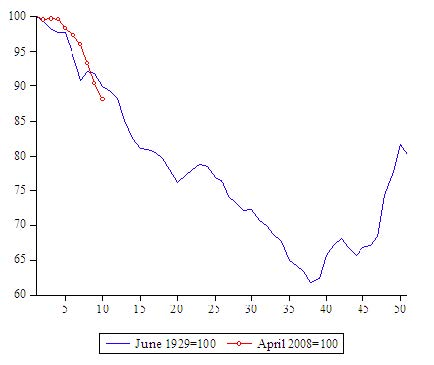
\includegraphics[width = 0.5\textwidth]{Economic_Rules_-_lecture_6_TBA-1.jpg}
Reasoning comes essentially in three forms, that in practice are used in conjunction
\begin{itemize}
\item \textit{Inductive reasoning} - Piecing together a picture from the evidence available
\item \textit{Deductive reasoning} - deducing facts from simple truths 
\item \textit{Analogical reasoning} - picking an appropriate analogy to understand the world
\end{itemize}
Analogical reasoning is primarily used whenever a fast decision must be made (financial crisis) or when disagreements about what is needed for deduction, or what is good evidence for induction, makes it difficult to reach conclusions through the 'usual' methods. During the financial crisis the great depression became a useful analogy to determine which actions should be taken, similar fast-decision situations that are were used for analogical reasoning are.
\begin{itemize}
\item Pearl harbor $\rightarrow$ The Cuban missile crisis
\item 1918 influenza epidemic $\rightarrow$ 1976 swine flu
\item Exxon Valdez $\rightarrow$ 2010 gulf oil spill
\end{itemize}
Central issues in analogical reasoning are those of cherry picking (picking an analogy to justify actions) and 'ease of access bias' (some historical events are more widely taught, and may therefore be used as analogies when there are better analogies available). Some of this comes down to \textit{institutional memory} which is often established through libraries serving specific state organs. 
\epigraph{"History doesn't repeat itself but it often rhymes"}{\textit{Mark Twain}}
A more economic case of analogical reasoning is that between the gold standard and the eurozone. When the gold standard was established it was to bring back prosperity after WWI, while keeping states from spending more than feasible, thus ensuring democracy and peace. In the same way the eurozone was invented to ensure economic cooperation to the point where war would be unthinkable, and it would bring Germany into the heart of European cooperation. Both systems would show to entail hard austerity measures to the countries not fitting well with the overall economic model on which the systems were build.
\subsubsection{Why economists need history}
\epigraph{“I think I’ve learned as much from studying the history of central banking as I have from knowing the theory of central banking and I advise all of you who want to be central bankers to read the history books.”}{\textit{Stanley Fischer}}
According to Stephen King, historical knowledge is needed because all market participants must be able to talk about risks in a 'big picture' framework. Without historical knowledge we run the risk of getting \textbf{financial amnesia} where central market players 'forget' the risks associated with specific trades, leading to mispriced assets, bubbles and crises. To a student studying history of economics it shows that major discontinuities are not so rare after all but the complacency has risen with the \textit{great modernization}.
\epigraph{"Zoom out, and that swan may not seem so black after all"}{\textit{Unknown}}
Economic history in other words teaches the importance of context, after all history is full of financial institutions developed to solve one problem that ended up being problems in themselves. Instead of narrowly considering our models, we must remember that our goal is to understand the real world. Economic history provides 'grounding' and prevents us from loosing touch with the world around us in the attempt to achieve technical skills - in fact it would be best to look at history before even trying to model the present.

\subsection{What makes a good applied economist?}
\epigraph{"[...] He must be mathematician, historian, statesman, philosopher—in some degree. He must understand symbols and speak in words. He must contemplate the particular in terms of the general and touch abstract and concrete in the same flight of thought."}{\textit{Keynes}}
How comes the education in economics is so based on research, while leaving little place for multidisciplinary approaches? While doing a PhD learns you how to do scientific research, few economists actually need that skill set. As Keynes put it, the economist should be able to use almost every science, and balance approaches to learn what is important about the economy.
\subsubsection{Schiller \& Schiller (AES, 2015)}
S\&S takes a critical look at the tendency for economics to foster specialists with very little knowledge of other disciplines. They acknowledge that specialization has many advantages, but also see disadvantages in the way competition among economists lead them to have very little understanding of anything outside of their field. Keynes formulated his theory of \textbf{animal spirits} as an opposition to the probabilistic approach to model behavior. To him much uncertainty of economics was not a result of probabilities, but rather of the 'animal spirit' of humans, lending them to impulsive and optimistic actions. One of Keynes' major works is \textit{The Economic Consequences of the Peace} in which he analyzed the Versailles treaty (specifically the heavy reparations the Germans had to pay) and predicted the events leading up to WWII. In his book he use all sorts of different sciences and "showed an extremely broad, inductive, mode of inquiry"(S\&S) - traits which Shiller and Shiller also identify in those who predicted the financial crisis of 2007. 
\\ \\
This all brings into question of todays economics is to narrow in its view of the world - possibly we should focus more on preparing students to work in government, than in research. Very little work is done on the work of economists outside of research. A UK questionnaire from 2012 points to a need for more practical tools like 'ways to answer externalities', 'impact analysis' (did it work) and more guidance in how to use a model, rather than how to build one. Among the most answered categories of type of work were 'production of briefing material' and 'preparation of policy advice', so maybe more emphasis should be put on learning to synthesize evidence. 

Furthermore the participants noted that knowledge of institutions and their impact on policy was important, and that ad hoc problem solving often occurred. Data work is to some extent important, but more often in the sense that economists needed to understand applied econometric work, rather than doing it themselves. 
\\ \\
Dave Ramsden says there are two types of economists - those desired for academia, and those not. Economists focus on educating the former group, and thereby neglect the economics students who will end up working in regular jobs. Here demarcation lines between disciplines vanish and often 'more research needed' is not a viable option. Instead non-academia economists rely on socio-economics and good communication.
\paragraph{Ways of knowing} outside of academia economics, many ways of knowing are employed. A \textit{naturalist} approach would be statistical, but also used is the completely opposite anthropological approach. Often mixed methods are used, for example combining focus-group interview with large-N studies. A central skill is \textit{source criticism}.

\subsubsection{Reforming the curriculum}

Good teaching encourages reflection and critical thinking, but pressure on universities to get good pass rates forces 'teaching for the exam'. At LSE all undergraduates must take the course LSE100, which teaches multidisciplinary approaches to big questions like climate change, population growth and the financial crisis. The course gives skill in methodology (evaluate and interpret evidence), information (find, critically asses and manage information) and communication (construct coherent arguments and plan+deliver presentations).

On the student side, students must realize that education is two way communication. Lectures should only be one of several sources of knowledge, and often there are many answers to a question. In the end independence of learning and thinking is what sets universities apart from schools. 

\section{Part 3: PoS in practice}
\subsection{Experiments in economics; methods, methodology and PoS}
A scientific experiment is “a scientific procedure undertaken to make a discovery, test a hypothesis, or demonstrate a known fact.” according to the Oxford English Dictionary, or "“a method of investigating causal relationships among variables.” (Wikipedia). In brief it's a setting in which scientists elicit data through a controlled process. Experiments have been used for a long time, also in economics. David Hume writes about using 'careful and exact experiments' in 1739, however since then using experiments has fallen out of favor, and in 1985 Samuelson and Nordhaus wrote that 'economists unfortunately cannot perform the controlled experiments of chemists'. Friedman has written similarly to Samuelson in 1953. With the advent of behavioral economics this has begun to change again. We now generally have both \textit{happenstance} and \textit{experimental} data.
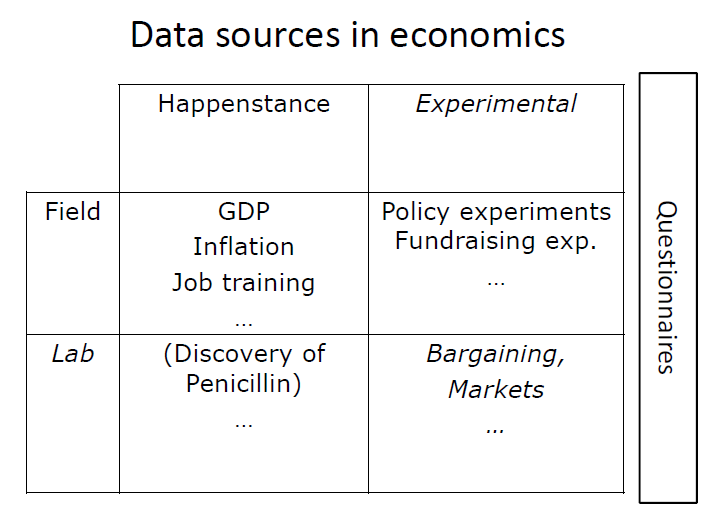
\includegraphics[width = 0.5\textwidth]{Capture.PNG}
Happenstance data generally makes it difficult to find clear causal relationships, and even more so when they're field observations. Recall Humes definition of causality in \ref{seq: causality} (in this slideshow the definition is attributed to Mills). This is seldom how experiments infer causality, instead we usually 
\begin{itemize}
\item manipulate the presumed cause, and observe the outcome afterwards
\item see whether variation in cause is related to variation in outcome
\item use various methods during the experiment, to reduce the chance that other factors are the true causes
\end{itemize}
There are many ways in which a lack of experimental control can seriously pollute scientific results. Therefore experiments are preferable, even though they're often very expensive and difficult to manage in social sciences. 

It's about 60-70 years since the first economist started running experiments on various topics in microeconomics. This has kickstarted "one of the most stunning methodological revolutions" (Francesco Guala) in economics (and maybe science as a whole). Even Samuelson, who previously thought economic experiments impossible, has stated that experimental economics is an "exciting new development". 
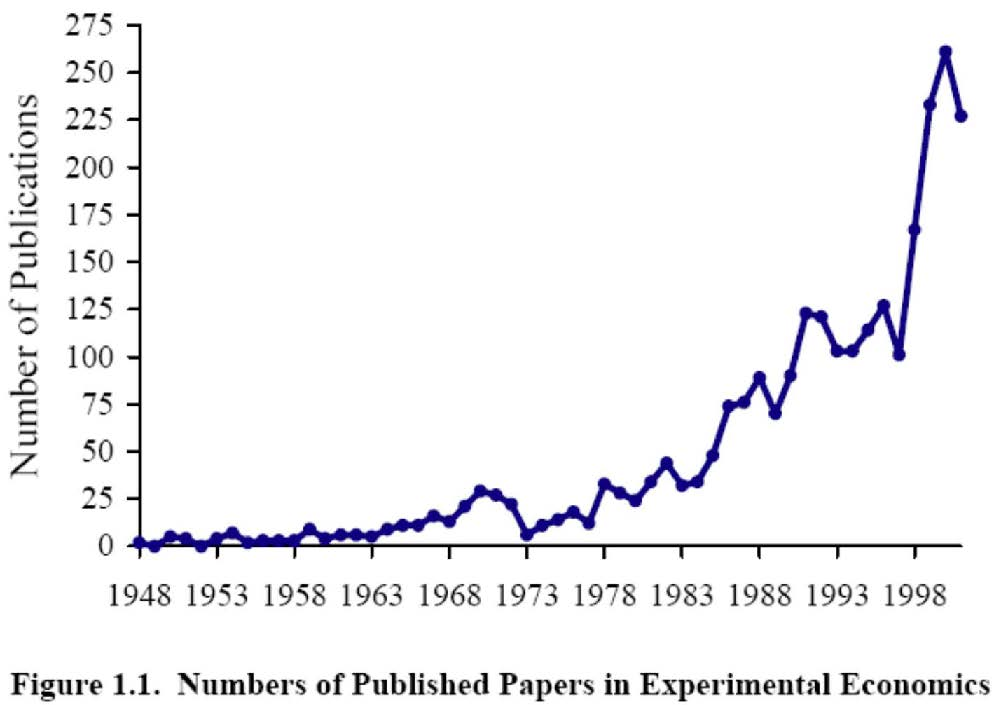
\includegraphics[width = 0.5 \textwidth]{Lecture_14_Experiments.jpg}
This new development has resulted in Nobel prizes for Smith, Kahneman, Selthen and Roth since 1994. At the core of experiments is the concept of \textit{control}, including controlling the background/environment of participants, and the institutions and possible actions in the experiment. Well specified experiments almost surely rule out issues of endogeneity, and thus allow better comparisons between theoretical predictions and the real world. Another huge gain is that experiments are \textbf{replicable} i.e. they can be attempted again in different settings or at different times. Smith, Croson and Gächter propose the following 7 purposes of experiments in economics:
\begin{itemize}
\item[1)] test theories
\begin{itemize}
\item in experiments we can implement conditions of a theory, and test if it holds. This will always be a joint test of the whole theory at once.
\end{itemize}
\item[2)] explore why theories fail
\begin{itemize}
\item With good control treatments we can identify which parts of experiments cause them to fail, and thus gives clues as to how we can improve our theories.
\end{itemize}
\item[3)] establish stylized facts for new theories
\begin{itemize}
\item This is closely linked to 2) - if we observe systematic deviations or reactions when repeating experiments, we might want to construct theories around these deviation, building theory from simple, testable 'truths'. Furthermore we can generate explorative results on unsolved questions and sometimes use experiments to select the relevance of multiple equilibria.
\end{itemize}
\item[4)] compare institutions and environment
\begin{itemize}
\item By having market structure exogenous we can investigate the effect of rules, regulation or similar in experiments.
\end{itemize}
\item[5)] generating policy advice from 'wind tunnel experiments'
\begin{itemize}
\item Instead of implementing policy at first (costly and risky) we can carry out wind-tunnel experiments of proposed policy to better understand its implications. For this to hold of course we need to consider the \textbf{external validity} of our experiments.
\end{itemize}
\item[6)] measure preferences
\begin{itemize}
\item Without inferring causality we can use experiments to measure parameters of preference w.r.t time, risk etc. while meeting the challenge of \textit{incentive compatibility}. 
\end{itemize}
\item[7)] teach students through experiments
\begin{itemize}
\item Lastly experiments can be used to teach students about simple economic principles, or illustrate where they fail.
\end{itemize}
\end{itemize}

\subsection{Experiments, realism and the complementarity of empirical methods}
Experiments can be conducted in a number of settings, i.e. different locations and different participant pools. Harrison \& List have gathered the following incomplete taxonomy of experiments
\begin{itemize}
\item Lab experiments - usually employ student participants, an abstract setting and fixed rules.
\item Artefactual lab experiments - employ a non-standard subject pool, for example game theorists.
\item Framed field experiments - is similar to the artefactual experiments but use 'field context', i.e. fishermen playing the public goods game.
\item (natural) field experiments - takes the lab to the field by observing someone who's naturally playing a game that is somewhat controlled.
\item natural experiments (quasi experiments) - experiments that take place coincidentally, often policy changes. 
\end{itemize}
\subsubsection{Objections against experiments}
A common critique of experiments is that they're artificial, because the participants are students, 'WEIRD' (western, educated, industrialized, rich and democratic) and also because samples are small and stakes are low. Of course none of these are fundamental objections, as we could easily fix them by hiring different participants or increase stakes. 

Another common critique is that experiments are 'unrealistic'. This is essentially a question of external validity - does experiments have \textbf{external validity} even when they have near perfect \textbf{internal validity}? This is a real concern and among the reasons why participants might not behave as they would in the real world are
\begin{itemize}
\item Scrutiny - participants know they're being watched
\item Anonymity - participants are anonymous to the researchers and their co-participants
\item Context and stakes - are often very different in the lab compared to the real world
\item Selection into experiments - participants self select into experiments
\item Restricted choice set and time horizon - participants take these things into account when making choices
\end{itemize}
Especially concerning is whether these issues lead to overestimation of effects of 'fairness' and other moral goods. As an objection, one could state that lab experiments are just as much 'real world' as anything else, but still the question of external validity would stand.
\epigraph{“The laboratory [is] a place where real people earn real money for making real decisions about abstract claims that are just as “real” as a share of General Motors.”}{\textit{Vernon Smith}}
For models that generalize behavior, experiments are nonetheless valuable, as any generalized model, should hold in any special cases which it claim to cover, including lab experiments. 
For an experiment to travel well in the real world, it needs a high degree of \textbf{parallelism} (it should be isomorphic to the real world), that is it should in all relevant ways be parallel to the 'real world'. Skeptics of a specific experiment should therefore try to argue that its conclusions does not travel well from lab to society. Of course this critique would only encourage more experiments with a higher degree of sophistication to be undertaken, thus failing at critiquing experiments as such. 
\\ \\
An important question is whether experiments should be realistic, or as with models, we should consider simplicity a virtue. In the end the answer depends on the purpose of the experiment. If one is trying to test a certain hypothesis it makes sense to leave out unimportant elements (like doing physics in 0 gravity), but if the purpose is to do 'wind tunnel' testing of a policy it makes sense to construct the experiment as close to reality as possible. 

\subsubsection{Experiments and induction}
Experiments are inductive in nature - they can never prove that they will always provide the same results. Therefore we rely on faith in the regularities we observe to persists, when building theory around experiments. This holds for natural experiments as well, and the debate of the external validity of empirical research carried out in the western world is ongoing in \textit{development economics}. 
\epigraph{“…the question of external validity, like the questions of inductive inference, is never completely answerable”}{\textit{Campbell \& Stanley}}
Similarly we can never know how well empirical findings generalize from the specific population and setting they were performed in to other settings. We can never substitute happenstance data, fields experiments, surveys or theory for experiments as each type of research works together and bring unique contributions. 
\\ \\
Alternatives to experiments include research like 
\begin{itemize}
\item Natural experiments, for example random assignment to study groups or charter schools with many applicants
\item Regression discontinuity designs - exploit discontinuities caused by policy to compare before/after or regional differences
\item Difference-in-difference approaches - use this or other statistical techniques to remove noise, measurement error or biases. 
\item Use quasi random variations in time 
\item Structural estimations
\end{itemize}
Not to forget that purely correlational studies can still be interesting, as they inspire future research. The strongest kinds of research usually compare or combine data from various settings, i.e. lab+survey or register+survey+lab, although this is never a sufficient condition for good research - plenty of bad research employ a multitude of data sources. 
\subsubsection{Case study: peer effects in lab and field}
Peer effects happen when behavior of individuals 'spill over' on other group members. This is notoriously difficult to measure, because questions like "is the causality going from $i$ to $j$ or opposite?", "are both affected by some background variable?" and "are self selection at play?" cannot be answered without some degree of control. In essence what's missing is the \textbf{counterfactual observations} of some group not existing. 

\paragraph{Falk \& Ichino (2006)} use a lab experiment to study peer effects in the workplace. They employed 24 high school students to perform a simple task, some were assigned to a treatment where they would sit in the same room, but weren't allowed to co-operate, while others we placed alone in rooms. What they find is that a 10\% increase in peer output gave a 1.4\% increase in ones own output.

\paragraph{Mas and Moretti (2009)} acquired scanner data from a US supermarket chain as foundation for their field experiment. the general idea is that the employees vary in productivity, and who's at work changes through the day. They measure productivity by the number of items scanned over a fixed time, and estimate the change in coworker $i$'s current productivity change with the permanent productivity of other coworkers. Very similar to Falk and Ichino they find that a 10\% increase in coworker productivity increase own productivity by 1.5\%.
\\ \\
In 2015 Herbst \& Mas carried out a meta-analysis of research in peer effects. With a sample of 11 lab experiments and 23 field studies they conclude that results are generally consistent and very similar between lab and field studies. 

\subsection{Economics and psychology}
Behavioral economics is the intersection of economics and psychology, a field which aims at founding economic models in psychology and behavior. Traditionally models are constructed with assumptions of coherent, stable preferences, which can be ordered by a utility function. Based on these traits they behave rationally and maximize their utility. Often utility is assumed to be individual, i.e. it doesn't depend on the utility of others - a philosophical point traceable to Adam Smith.
\\ \\
Behavioral economics deal with the anomalies that arise when making the traditional assumption, often by first observing anomalies in happenstance data, to then later explore why a certain phenomena happens in the lab. The field works in much the same way as lab-researchers, beginning from existing theory and possibly conflicting evidence. From this behavioralists study the anomalies, and develop new theory to incorporate them. Most 'puzzles'/anomalies can be categorized as one of the following
\begin{itemize}
\item non-standard preferences - the study of what preferences look like in real life
\item non-standard beliefs - the study of how people form beliefs, and if systematic biases are present
\item non-standard decision making - the study of decisions that deviate from the predictions made under perfect information and rationality
\end{itemize}
One major anomaly is the assumption that individuals utility is pure self interest - for example 89\% of US households donate to charity and voluntary labor make up approximately 9 mio. full time jobs each year. A good framework to study this is the 'ultimatum game' where two players take turn offering splits of a fixed amount between them. Theoretically this should result in a split of $(s,1-s)=(1,0)$ if agents were rational, but in experiments most senders offer 30-50\% of the total sum, and receivers typically reject any offer lower than 20\%. Among the proposed explanations is that participants don't understand the game, or that stakes are to low - both of which has been refused by rerunning the experiment with different setups. One could then take it as evidence that participants are altruistic, but given the reactions of the responders, the proposers(1st movers) behavior is actually quite consistent with self-interest and rationality. It seems that what's happening is that the responder(2nd mover) feels 'unfairly' treated if he gets a low share of the split. Why this happens is unknown, but possible answers include envy, wanting to punish unfair actions and status concerns. 
\\ \\
To explain the results from the ultimatum game Fehr \& Smith have proposed a utility function that contains inequality aversion. If the split is unequal, people loose utility at different rates, depending on who gets the most, mathematically
\begin{align*}
u_i(\cdot) &= x_i - \alpha_i \text{max}[x_j - x_i, 0] \\
& -  \beta_i \text{max}[x_i - x_j, 0]
\end{align*}
Another interesting question in BE is the importance of reference points. For example Kahneman et. al. have assigned coffee mugs worth \$ 5 to half of a participant pool. Afterwards the participants could trade mugs with each other. We would expect them to converge to an equilibrium value where those who wanted the cup the most got it, and since mugs were assigned randomly, the proposed prices from buyers and sellers should therefore be the same. Instead Kahneman found that the willingness to pay among buyers was \$2.30, while the sellers demanded an average of \$ 5.25 to sell. This and similar studies have lead researches to believe that people use a reference point, or status-quo, relative to which they evaluate outcomes. Combining this with a distaste for changes or 'loss aversion' gives much better predictions than the ordinary theory. 
\epigraph{"Pain … is, in almost all cases, a more pungent sensation than the opposite and correspondent pleasure"}{\textit{Adam Smith} on loss aversion}
A third question in BE is that of time-inconsistent behavior. If you ask people whether they prefer fruit or chocolate in a week, most will say fruit. If however you wait one week and then ask people what they prefer on the day, most say chocolate. This has led to the development of \textbf{present bias} theories, most notable of which is probably the $\beta - \delta $ model, which discounts the future more heavily than the present. Similar to this is the notion of consistent biases. When people are asked to give estimates of how they fit in the distribution of a population on some parameter, they often 'guesstimate' themselves to be above average, although of course statistically around 50\% should be below. This is often attributed to problems with \textbf{Bayes-updating}, that is using Bayes rule to correctly calculate probabilities. Dophem et al. asked 1012 participants in Germany what the probability of rain tomorrow is, if it rains 10 out of 100 days, weather forecasts have an 80\% success rate in predicting the weather, and it's been forecasted that it will rain tomorrow. This is simple to calculate as 30.8\% with bayes rule, yet no participants gave the correct answer. 

\subsection{Behavioral economics, economic policy and paternalism}
This lecture asks how we should handle innovations in modeling and policy advice from behavioral economics from a PoS perspective. The inventions include reference points $u(x|r,s)$, social preferences $u(x_i, x_{-i}|s)$, present bias models and more. We categorized them in 
\begin{itemize}
\item \textbf{non-standard beliefs} - like problems with bayes updating/conditional probabilities, biased probability estimates and projection bias (guessing wrong about how people react to big changes in the future)
\item \textbf{non-standard decision making} - such as limited attention and menu/context effects.
\end{itemize}
Most new alternative models have in common that they introduce additional parameters, and thereby allow for additional degrees of freedom. This raises the question of where to stop: when are models sufficiently detailed that adding more layers brings unnecessary complication, after all parsimonious models are valuable. 

Probably what we should measure models on is their ability to "account for a range of systematic deviations from the standard models" without being dependent on context. They should furthermore be usable for at broad range of applications in policy.
More often than not the new more complex models are difficult- if at all solvable. They often bring new puzzles instead of answers.

\subsubsection{Paternalism}
One major question that has risen with behavioral economics is if people act against their own self interest in certain situations, and as a follow up to this, how do we measure welfare with irrational agents. Unlike in traditional economics where policy is usually harmful because people have stable preferences, behaviorist agents switch their preferences without reason (?) so we loose the benchmark of rationality to test against, and whether or not to even measure welfare becomes a debatable question since it implies defining what is good for individuals, even though they may actually want to act 'inefficiently'. As an example we can consider present biased individuals as consisting of two 'selves' which make conflicting choices. This generates 'internalities' on the individuals themselves, leaving the question of what 'self' to measure the welfare of open. Ultimately we might want to implement policy to counter these internalities in the same way as we do with externalities - should we for example implement policy to prevent advertisers or firms from taking advantage of behavioral traits?
\\ \\
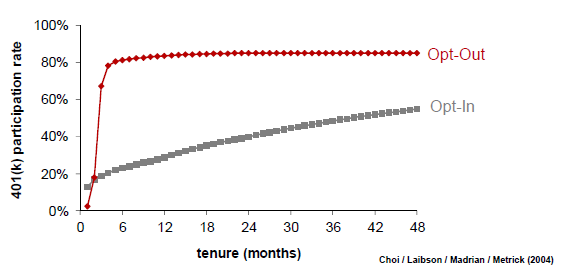
\includegraphics[width = 0.5\textwidth]{optinoptout.PNG}
A very concrete example of this dilemma is whether or not the state should dictate for employers whether or not their retirement savings schemes are opt-in or opt-out systems, as this makes a large difference to enrollment rates. Most people believe they save to little for retirement, so implementing such rules would probably help many, but on the other hand it's clearly paternalistic. In reality however it doesn't change the option-space of individuals so it could also be argued that the policy would be libertarian. This has lead Thaler \& Sunstein to coin the term \textbf{Libertarian paternalism} - the idea that such 'nudging' policies can be implemented to correct for behavioral traits, thus making many better off, while hurting no-one (freedom of choice is preserved). 
\end{multicols}
\pagebreak
\footnotesize
\begin{table}[]
\centering
%\caption{My caption}
%\label{my-label}
\begin{tabular}{@{}p{8cm}p{8cm}@{}}
\toprule
\multicolumn{2}{c}{Libertarian paternalism +/-}                                                                                                                                                                                                            \\ 
\multicolumn{1}{c}{\textbf{(+)}}                                                                                                   & \multicolumn{1}{c}{\textbf{(-)}}                                                                                                            \\ \midrule
\textcolor{blue}{1)} Systematic deviations from efficient outcomes are costly to society                                                     & \textcolor{blue}{1)} Bureaucrats are not necessarily incentivized to make good decisions for citizens. Neither do they have all relevant information. \\
\textcolor{blue}{2)} It's an alternative to more invasive policies.                                                                          & \textcolor{blue}{2)} It's a slippery slope towards more restrictive regulation.                                                                       \\
\textcolor{blue}{3)} Policies often specify a default situation anyways, so we might as well set the rules with the best outcome for people. &                                                                                                                                  \\ 
\textcolor{blue}{4)} Even without 'nudging' people have to make choices & \textcolor{blue}{4)} It encourages passiveness, it's better to force people to make a choice
\\
  & \textcolor{blue}{5)} People might become used to being nudges so much that it looses its effectiveness 
\\
  & \textcolor{blue}{6)} One nudge might not be enough, if setting 'opt-out' as default for 401(k)'s donations we then also need to set rules for the default savings rate, asset allocation etc. This might do more harm than good.
\\
\bottomrule
\end{tabular}
\end{table}
\normalsize
\begin{multicols}{2}

Typical instruments for libertarian paternalistic policies (a.k.a 'nudges') include
\begin{itemize}
\item defaults
\item information disclosure, framing and labels
\item reminders
\item cooling-off periods
\item self-commitment devices 
\item (constraining choice sets)
\end{itemize}
Nudges can be applied to a range of different problems, for example consumer protection, environmental issues, in taxation, health-care and a whole number of others. A canonical example is that of organ donation. Here countries with opt-out schemes for organ donation see a much higher rate of effective consent to donation than those with opt-in schemes. Altmann \& Traxler conducted an experiment in 2014 where they send out reminder texts for dental checkups, which resulted in much higher turnup rate for preventive checkups. They furthermore note that a majority of patients who doesn't get reminder would like to get them. 

Similar results have been found in tax-policy, where the difference in framing between a 'tax-bonus' and a 'tax-rebate' substantially increased the degree that went towards consumption. 

\subsection{Economics, ethics and scientific (mis)conduct}
Ethics (aka moral philosophy) is a branch which systematize, defends and recommends concepts of right and wrong conduct. Philosophical ethics investigates how humans should live and what is right and wrong. In PoS we focus on the ethics of conduct in science and economics in particular. Economists are humans like anyone else, and therefore face conflicts of interest and are influenced by their own morals and ethics when conducting research. A well functioning scientific field is therefore dependent on the ethical conduct of its actors, as well as a scientific process structured to minimize conflicts of interest. 
\\ \\
As economists, luckily we're trained to study the effect of incentives on behavior, so we should be good at identifying potential issues with incentives in out science. For example when we appear as experts, we have an inherent incentive to give advice that benefits ourselves, or in academia we often meet strict demands for publications, which incentivizes mono-culture in our science. 

As experts, we advice policymakers and companies in their economic decisions. The advice we give/are asked to give might affect what research is undertaken, our personal morals or ethics might influence our advice or we might even be persuaded to give advice that is in accordance with our own financial interests. This problem is of course not limited to economics, many other fields of science are likely to be influenced by the surrounding society. Possible solutions could be to forbid scientists to earn money through consulting, or forbid scientists from consulting altogether or forbid private/(public?) funding of research. Both of these are of course extremes and would have severe downsides. Instead the more viable solution is to disclose conflicts of interest as best as possible. 
\\ \\
In academia we face incentives similar to the ones in the rest of society, including our intrinsic motivations (to teach and do research), and incentives of financial and social sorts. Especially for science the publication- and research output measures are strong incentives to do research that is eligible for the highest ranking journals, even if these have a narrow focus. As an economist the normal career ladder goes from M.Sc. through a Ph.D. degree and continues through the ranks of university employees (Post-Doc, ..., full professor). In all stages ones career success is strongly linked to ones research success and publication records. For example there are around 700 applicants for each opening as 'adjunkt' at KU, making good publication history extremely important. In the same way external funding is often awarded on the basis of publication history. 

We might also ask what constitutes a good publication - and even though we would like the answer to be 'novel knowledge' or 'practical impact' the truth is often, that in the minds of researchers the quality of publications can be measured by the ranking of the journal they were published in. 
\\ \\ 
The publication system has several openings for misaligned incentives, for example in the peer review process, in the crediting of coauthors or in the bias against 'non-results'. Specifically the peer review system implies that the best qualified reviewers are also to some extent 'competitors', giving them incentives to disapprove of good research. 

Likewise it might be tempting to add coauthors that haven't made significant contributions, as long as they also add one self as coauthor on their article. 


\subsection{Economics, ethics and scientific (mis)conduct II}
\paragraph{Plagiarism} is an eternal problem in science, but it's not only necessarily the fault of the researchers, the system which encourages high-frequency publication might also play a role, and since the peer-review system is far from perfect, plagiarized work sometimes gets publishes. A nice example of this is the case of previous German minister of economic affairs  Karl Guttenberg, who managed to become minister and gain a doctoral title in constitutional law before being discovered as having plagiarized the entire thesis. 

Journals usually not only prohibit plagiarizing from others, but also from reusing old work without citations. This was felt by Bruno Fey (top 50 economist) in 2010, when they published four papers without cross-referencing, and without referencing similar work by other authors. In the end this cost him his position at the university of Zurich. 


\paragraph{False-positive science} or type-1 error publications, is the phenomena of papers seemingly finding significant effects, when in fact there are none. These arise from a number of sources, first of all results are far easier to publish than non-results, inducing a bias towards research that looks for significance. This combined with the flexibility allowed in data handling during the analysis - excluding outliers, selecting variables etc can in many ways alter results if they're not sufficiently robust. These incidences range from conscious 'p-hacking' to the less malignant unintentional incompetence. 

\paragraph{fabrication of results} is luckily rare, but does occur, for example in the case of Milena Penkowa. Her doctoral thesis wasn't approved in the first instance, but was later approved by a second external committee. Later when students had difficulties replicating her results, KU investigated and exonerated her of any wrongdoing (2008). Then in 2010 when more students were unable to replicate results, the case rolled and she lost her job. Many of her coauthors and students faced serious problems as well. 

A similar case in Germany, where whole datasets were made up cost Diederik Stapel 120 hours of community service after settling for the deal with his prosecutors. 

\paragraph{Solutions?} All of these cases highlight that science have problems with keeping incentives in line with what is considered 'good' science. The traditional remedies have been to improve training and control, but it might be that incentivizing replication studies and transparency is the real solution. 
\\ \\
One way to encourage transparency would be to force researchers to publish a 'pre-analysis' plan, specifying which hypotheses the scientist intends to test and how - thereby restricting the scientists degrees of freedom. Another example is to make it a requirement that scientists share their data - this is already happening in many journals.
\\ \\
\epigraph{“non‐reproducible single occurrences are of no significance to science”}{\textit{Karl Popper}}
Replication is the act of repeating previous studies, for example by reanalyzing previous studies, replicating graph by graph or by conducting meta-analysis of several papers in the same topic. \textbf{Conceptual replication} is when scientists collect new data on a already examined topic, to see if results are robust to changes in environment and sample, whereas \textbf{direct replication} also involves collecting new data, but then reruns the exact procedures from a previous paper. 

Replication serves to discover mistakes in original studies either intentional or unintentional. Unfortunately not very many replication studies are undertaken, because journals prefer novel findings, and researchers dislike 'ratting out' each other. In recent years things have begun to change, some nat-sci journals now require replication to print papers, and major initiatives have been undertaken in economics and psychology. For example psychologists have founded 'open science collaboration' which is a network of departments that replicated older studies from three journals. They found an average decrease in mean effect (compared to the original studies) of 50\%. Of the original studies only 36\% were replicated with significant results, whereas only 47\% of the original effect sizes were within the 95\% confidence interval of the replication effect size. So assuming there was no bias in the original results, combining original results and one round of replication left only 68\% of studies with significant effects.
\\ \\
In economics Camerer et al. replicated 18 experimental studies in 2016 in accordance with the predefined analysis plans published prior to the replication experiments. They found significant effects in the same direction as the original in 61\% of the cases, and an average replication effect size of 66\% of the originals.  

\section{Old exam sets}
Friedmans idea of positive economics says we should not measure a theory by the realism of it's assumptions, but instead by it's predictive capabilities. To him models should be chosen as prefered based on the following criteria: they should be able to predict previously unobserved data, they should be parsimonious (i.e. they should not overcomplicate things) and they should provide paths for future research. 
To Friedman the realism of the assumptions is not at all important. To Friedman economic theory should evolve to replace old theory with new one, when new theories provide better predictions, and indirectly when new theories can explain more with less (or the same with less).

Popper on the other hand is the creator of a strict concept of falsification. To him there is no way of science to present truths. He makes an essential observation, namely that the relationship between verification and falsification is asymmetric, at least concerning induction. Therefore scientists should pose new theories through leaps of imagination, while rigorously attempting to falsify already posed theories. Thus Popper would in the first instance say that for Friedmans method to be scientific, that the predictions should be easy to make, test and potentially use as falsification of theory. Secondly Popper might intervene that when assumptions are disregarded, this effectively works as immunizing stratagems through which new unrealistic assumptions can be added to preserve theories that would otherwise be falsified. 
\\ \\
Kuhn takes a completely different approach than Popper - being a physicist he is more concerned with the actual development of science, than the quest for demarcation rules to define 'good science' in a normative way. Kuhn's idea is that science evolves through paradigms, each of which are defined as periods of scientific consensus. Within paradigms 'normal' science occurs, and seminal articles, textbooks and the 'brotherhood of the field' lets the science develop through puzzle solving. However as more puzzles are solved anomalies will occur, and paradigms develop auxiliary theory that can explain these, or anomalies are ignored altogether. 





\end{multicols}
%\end{spacing}
\end{document}